\chapter{Related Work}

\index{Web Service}
\index{Web API}


\begin{figure}[!ht]
	\centering
  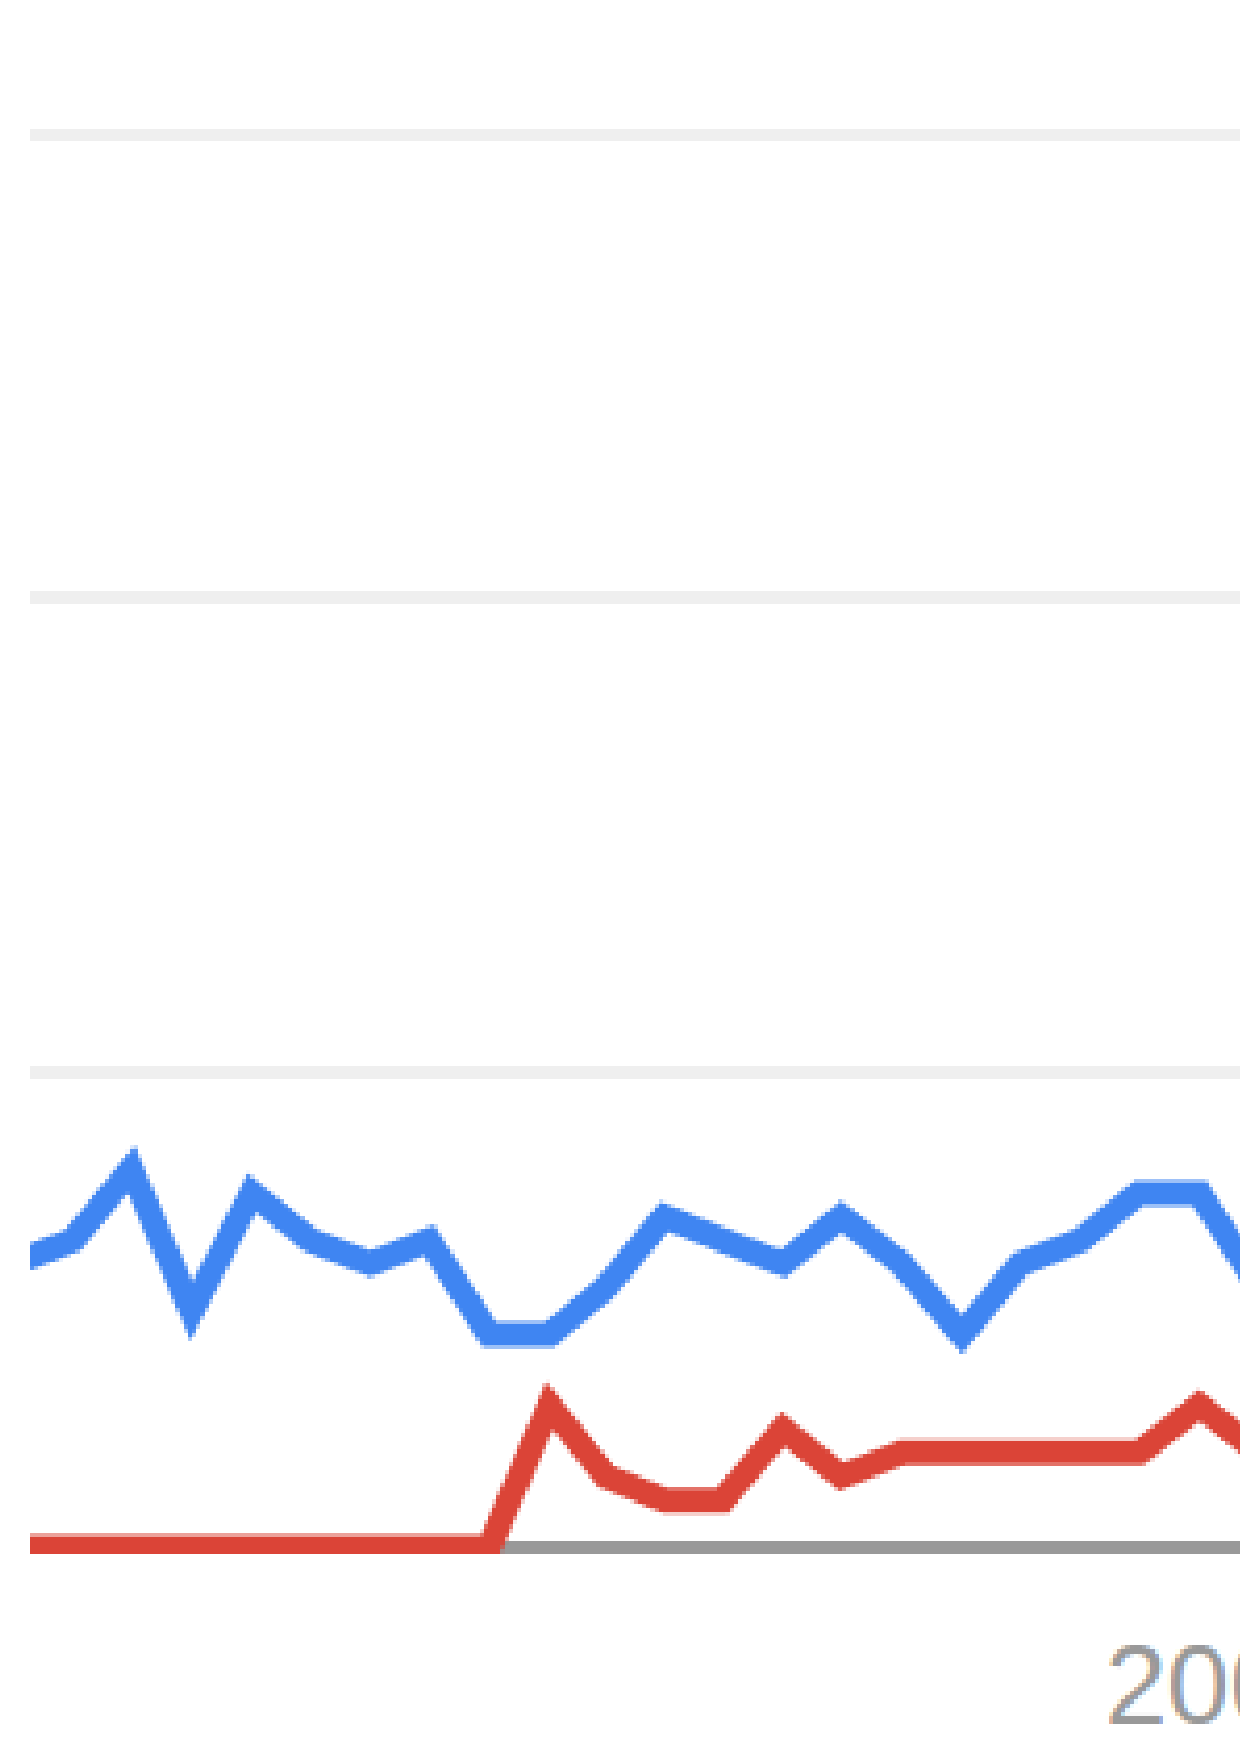
\includegraphics[width=0.9\textwidth]{figures/googleTrends_Rest-SOAP}
	\caption{Google Trends: "soap api" vs. "rest api"}
	\label{fig:googleTrends_Rest-SOAP}
\end{figure}
% Correlates with findings in http://www.slideshare.net/jmusser/open-apis-state-of-the-market-2011
\begin{figure}[!ht]
	\centering
  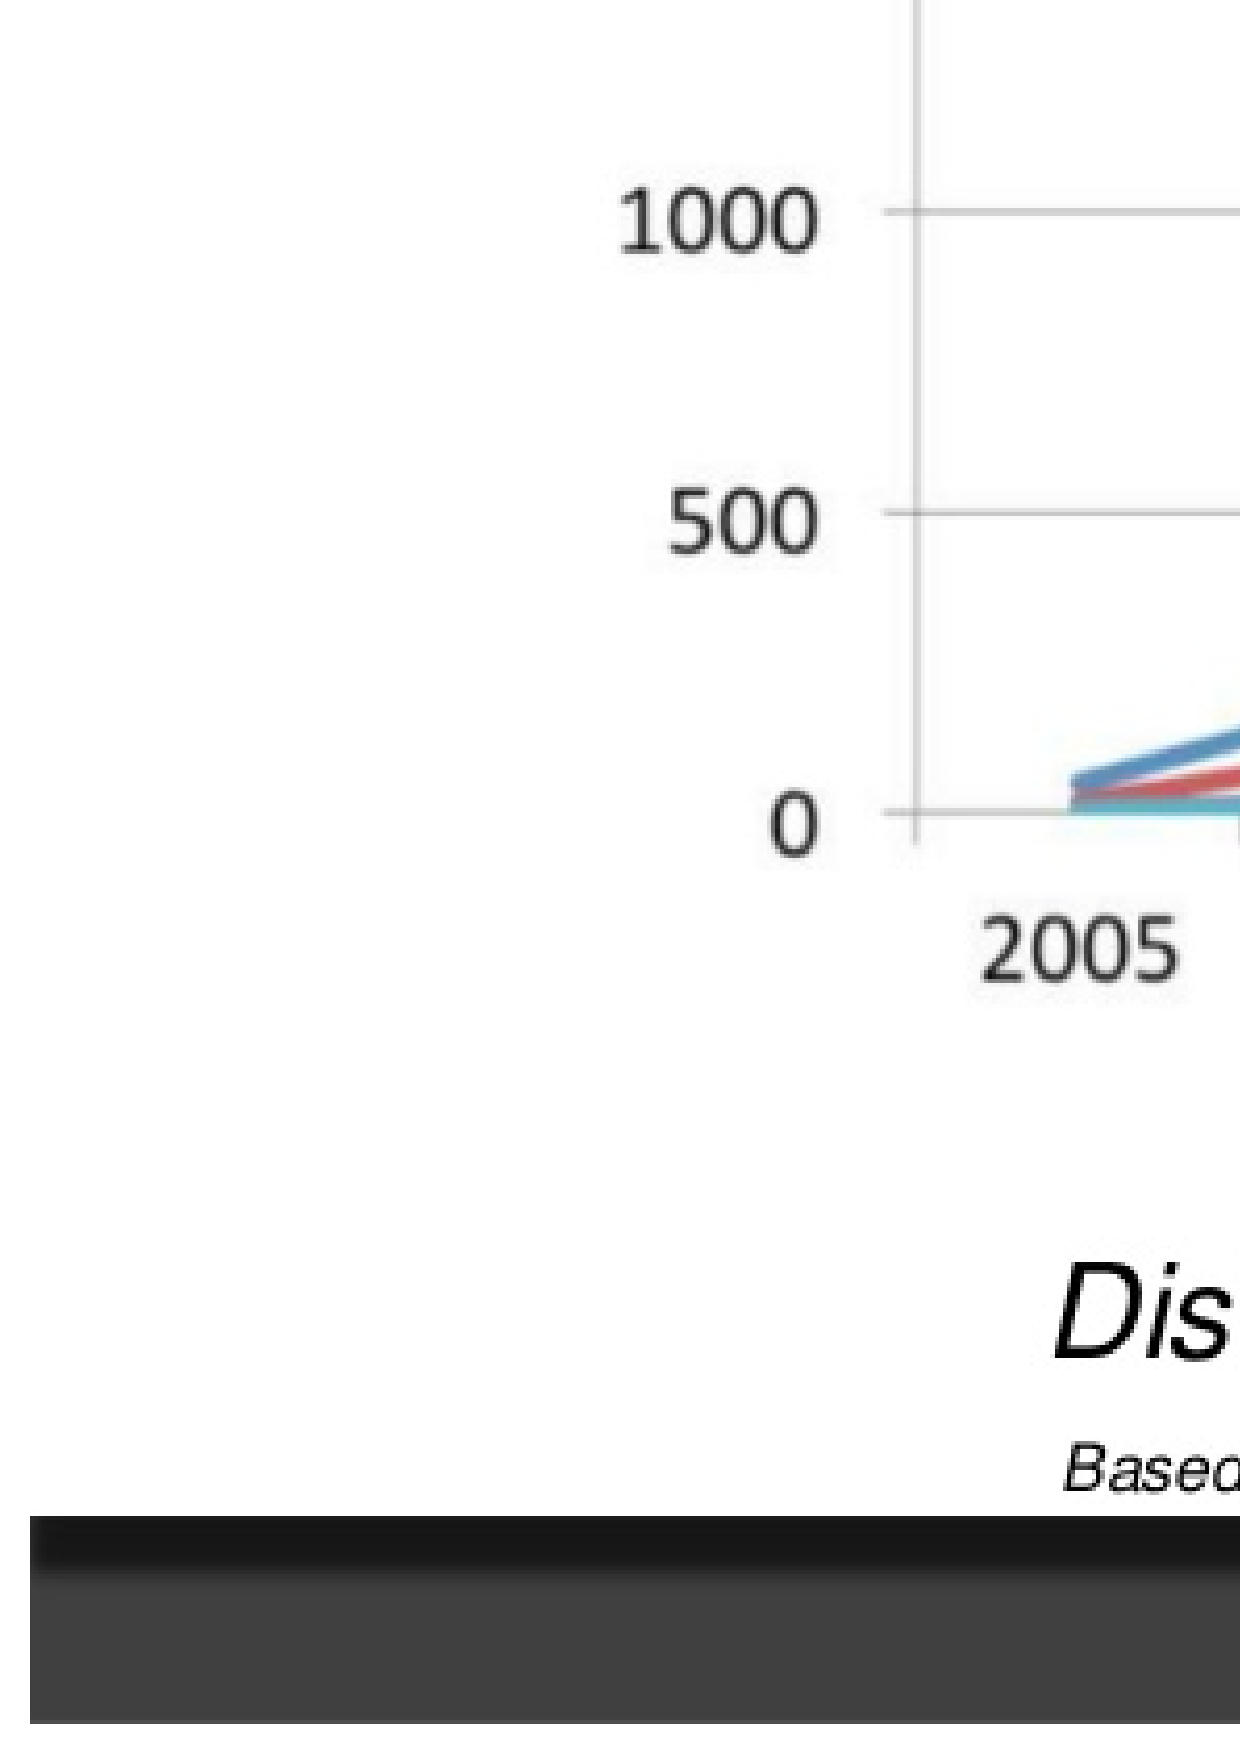
\includegraphics[width=0.9\textwidth]{figures/slide-11-1024}
	\caption{REST vs. SOAP: Simplicity wins again (John Musser, ProgrammableWeb, 2011)}
	\label{fig:slide-11-1024}
\end{figure}
Several different resources [Figure \ref{fig:googleTrends_Rest-SOAP}][Figure \ref{fig:slide-11-1024} (John Musser, ProgrammableWeb, 2011)] draw the same picture, an increasing popularity of REST over SOAP by an order of magnitude and a exponential growth of the number of accessible Web API's.


Web APIs are Web accessible endpoints for users to invoke.
With the wide adoption of Service-oriented Architecture (SOA), we see an increasing number of Web accessible services and their compositions.\cite{conf/icws/HuangFT12}

Twelve Theses on Reactive Rules for the Web\cite{10.1007-11896548_63}:
This article investigates issues of relevance in designing high-level
programming languages dedicated to reactivity on the Web. It presents
twelve theses on features desirable for a language of reactive rules tuned
to programming Web and Semantic Web applications.
% MY NOTES: they argue with soap and expect it to stay. They expect web sites to inform each other about update requests. we are taking one step further and provide events to whomeever wants to receive them while being greedy about receiving events. give them to meeeeh my prciouzzz eventz!
% 1. High-level reactive languges are needed, ECA rules well-suited to specify reactivity
% 2. Reactive Web rules should be processed locally and act globally through event-based communication and access to persistent Web data
% 3. Events are best exchanged directly between Web sites in a push manner
% 4. Events are volatile data and should be kept distinct from persistent data.
% 5. Recognizing composite events is essential for a reactive Web language. Composite events are conveniently specified by (event) queries. There are (at least) four complementary dimensions to event queries: data extraction, event composition, temporal conditions, and event accumulation --> Future Work (CEP), data extraction already implemented
% 6. A data-driven, incremental evaluation of event queries is the approach of choice
% 7. Data from persistent Web resources plays an essential role for Web reactivity. A reactive language thus should embed or build upon a Web query language.
% 8. The Web is a dynamic, state-changing system. Reactions to state changes (events) through reactive rules are state-changing actions such as updates to persistent data. Reactive rules are needed where compound actions can be constructed from primitive actions.
% 9. Development and maintenance of reactive rule programs can be considerably supported by structuring mechanisms such as: branching in rules, deductive rules for event queries and Web queries, procedural abstractions for actions, and grouping of rules. --> Future work, attach several conditions and their actions branches to one event instead of creating rules for each of them. EC^nA^n. (Though procedural abstractions for actions already implemented, defining complex actions to be reused by rules)
% 10.Identity of data items is an issue for reactive languages due to their ability to react to changes of data objects on the Web. (we had surrogate identity though discarded the concept again... stupido)
% 11. Meta-programming and meta-circularity, that is, the ability to use rules to exchange and evaluate (other) rules, are needed in some important cases. (quite artificial for our scenarios)
% 12.Reactivity in the Web’s open and uncontrolled world requires language support for authentication, authorization, and accounting. (phew... let's let others go there)


% Web Services – Opportunities and Challenges
% NICOLETA DAVID, CLAUDIA-GEORGETA CARSTEA,
% IOAN-GHEORGHE RATIU, LUCIAN PATRASCU, DANIELA DAMIAN
%Web Services term refers to available programmatic interfaces that are used in the World Wide Web for application-to-application communication.

% An approach to develop a layered architecture from software engineering, principles was proposed by Gerber et al. [23], referred to as the Comprehensive, Functional, Layered (CFL) architecture for the Semantic Web. C
 % - Gerber A., van der Merwe A. and Barnard A. Towards a Semantic Web Layered Architecture. In Proceedings of IASTED International Conference on Software Engineering, (SE2007), Innsbruck, Austria. IASTED 2007. ISBN 978-0-88986-641-6, pp. 353–362.

% http://benchmarksgame.alioth.debian.org/u64/benchmark.php?test=all&lang=java&lang2=v8&data=u64 seem to back our findings
% https://www.paypal-engineering.com/2013/11/22/node-js-at-paypal/ as well
% https://vividcortex.com/blog/2013/12/09/analysis-of-paypals-node-vs-java-benchmarks/ interpretes above results:
% My guess is that Node is encouraging good programmer practices in terms of scalability, and Java less so. In other words, programmers probably have to work less hard to avoid bad scalability bottlenecks in Node than in Java.


% XML SOAP WSDL UDDI RDF OWL
% microformats: xhtml rss

% http://www.w3.org/TR/ws-gloss/: A Web service is a software system designed to support interoperable machine-to-machine interaction over a network.
% http://www.informationweek.com/from-edi-to-xml-and-uddi-a-brief-history-of-web-services/d/d-id/1012008?
% -> Common Object Request Broker Architecture, Distributed Component Object Model, Unix Remote Procedure Call, and Java Remote Method Invocation. Each of those technologies failed to gain significant market share or enough momentum to succeed.
% CORBA , RMI
% XML officially became a standard in February 1998, when the World Wide Web Consortium announced that XML 1.0 had reached draft recommendation status: suitable for deployment in applications.
% SOAP won over WDDX (Web Distributed Data Exchange)
% SOAP 1.0, its specification for a standardized message-passing protocol based on XML.
% REST
% TODO dienste services WebAPI belegen mit referenzen wo begriff wie gebraucht wird
% Begriffe festnageln, definieren

% \cite{journals/itpro/BarrosD06}:
% The Rise of Web Service Ecosystems
% An increasing number of organizations are turning to service-oriented architectures (SOAs) to consolidate and repurpose legacy applications and combine them with new applications.
% A vendor-driven push for middleware based on the Web services standards stack is fueling this trend (Sanjiva Weerawarana and colleagues.
% Web Services Platform Architecture: SOAP, WSDL, WS-Policy, WS-Addressing, WS-BPEL, WS-Reliable Messaging, and More, Prentice Hall, 2005).
% This stack provides infrastructure for exposing application logic over the Web using the “software as a service” metaphor.



% \cite{10.1109/ICSS.2013.16}:
% The services and their correlations can be treated as a complex system with self-organize and continuous co-evolution properties, which is called service ecosystem.
% In service ecosystems, dynamic factors are general and may affect the performance of the whole system by spreading through the correlations.
% There is little systematic research on the effects of dynamic services while this topic plays a crucial role in the managing and controlling of service ecosystems.
% The transformation from traditional industry model of software to SaaS (Software as a Service) greatly changes the academic and economic domain of software, which brings about the prevalent research trend of service science [1].
% Web service is a typical kind of delivery method for SaaS, fueled by protocols and technologies (WSDL, REST, UDDI, BPEL, and SOAP etc.) [\cite{journals/itpro/BarrosD06}, 3]
% As the users’ needs become more specific and complex than ever before, it is a must for services to interact with each other to exchange control data and information. 
% There is little systematic research on the effects of dynamic services while this topic plays a crucial role in the managing and controlling of service ecosystems.
% So in this paper, we designed a research framework for researching the dynamic factors in service ecosystems.
% -> No measurements, would be interesting

% \cite{10.1109/MIC.2008.92}
% The Web is now programmable.
% This fact has been facilitated and accelerated by Web data’s availability as structured XML feeds (such as RSS and Atom) and by the externalization of Web application interactions through application programming interfaces.
% Indeed, most new Web sites and applications expose either data feeds or more advanced APIs, such as Representational State Transfer (REST) services or the Atom publishing protocol (AtomPub).
% Currently, the primary manifestation of the programmable Web are mashups.
% Mashups combine views, data, and logic from existing Web sites or applications to create novel applications that focus on situational and ephemeral problems.
% Developers are now using various Web APIs to create a plethora


Data and functionalities in the web were always accessible via web services, whatever this means.
reengineering of services in the beginning
with standardised REST API's we got to Web API, easy access and understandable


The fast evolving web has brought up a trend towards easy to master interfaces to services, the so called Web APIs.
They do not only provide access to mere services but whole applications that allow access over Web APIs.
These trending Web APIs benefit from a RESTful architecture which predominantly uses HTTP and thus relies on the most basic and powerful operations and the basis of the Web itself, the HTTP protocol. 

% TODO Enough on Web API's?

% quick (handling/mastering) accessible services and even whole web applications through so called Web APIs.
% Web APIs provide powerful tools to govern data and functionality in the web independently of any user interface from the service provider.
% The relatively
% Allowing access to these services via API is increasingly popular and allows to mash up these services

% Practically all services flood the user with events
% The web should be event driven, that's why we need an engine that deals with events and makes the web reactive
% There's still the challenge of filtering
% What's important to whom
% Plus the user needs to have tools to combine and add programmability to the combination,( such as conditions, selection of provided arguments and so on)

% % TODO Event Trigger
% \index{Event}
% \index{Event Trigger}

% % TODO Actions
% \index{Actions}

% % TODO engine
% \index{Engine}


% % TODO Webhooks
% \index{Webhooks}

% TODO Categorize Related Work!

\index{Mashups}
Mashups combine information and functionality of more than one web service in a single place.
The mashing up of such web services allows data to be enhanced with new informations, processing / refinement of the information, or even ways to interact with them, e.g. through Google Maps.
Simple functions from different sources can be combined into more powerful ones, which influence data and services in a way their founders eventually didn't even think of.
Web service mashups have been developped ever since services in the web started to exist and were accessible in a more or less convenient way.
We introduce Paul Rademacher as an example for how recent the invention of web service mashups are.
He's one of the first inventors of such a web service mashup.
In the same year after Google Maps came up in 2005, he invented a site\cite{wwwRademacherOne,wwwRademacherTwo} that displayed Craigslist houses on a Google Map.
With no Google Maps API at that time, he needed time and skills to reverse engineer Google Map's functionalities.


A large number of such "static" mashups were and are still developped.
They are static in the way that they aggregate a fixed (and mostly low) number, of either data or functionality resources, to provide an enhanced resource in a specialized domain.
Of course Mashups can be mashed up again, to provide even more sophisticated functionality and data.
Some latest example Mashups, taken from the ProgrammableWeb\cite{wwwProgrammableWeb} collection, are:

\begin{itemize}
  \item Wifi and Plugs\cite{wwwWifiAndPlugs}: MapBox, Google Docs and Import.io API's used to display where Wi-Fi and plugs are available in London.
  \item MapLight\cite{wwwMapLight}: GovTrack.us and OpenSecrets API's used to combine political results with financial contributions to show how capital contributions affect voting.
  \item Shared Count\cite{wwwSharedCount}: Facebook, LinkedIn, Pinterest and Twitter API's used to display informations about how well spread a URL is on social media sites.
\end{itemize}

In the past few years, research and development for platforms to allow users to flexibly mashup Web APIs got attention.
% Web API mashups
With IFTTT and Zapier, two platforms have evolved out of this process.
Users that register on those platforms are provided with a multitude of Web API functions that act as event triggers and such that are used to execute actions.
The user is then free to combine these event triggers and actions in the way it suits best, creating helpful Web API mashups on their own.

% Since this is a quite new field the why and how is hidden from the research.
% you need events
% you need rules / rule language

% TODO REST paper, Craigslist artcile / Paper



\index{Rule}
\index{Engine}
\index{Rule Language}

It turns out that Web API mashing up is not able to bring reactivity to the web.
They are merely aggregations of services that only provide data or functions but no write possibilities such as web applications provide.
% only limited functionalty
% limited parametrization
% often only read / new aggregation / no writes
% TODO find mashup that does writes in a system! (not existing right?)

Thus 

% TODO
% To allow user-defined Web API mashups, a rule language is required which is capable to express ECA Rules. 


% TODO
% ECA
% \index{ECA}

%TODO Table with categorization of Rule languages

Several different rule languages have been developped for different purposes over the last years and they vary grately in their purpose.
% terms of usability for ECA Rules together with Web API mashups.
A compilation of research on different emerging rule-based languages and technologies \cite{2009-Paschke_Boley-RCER.pdf} gives an oveview over such efforts.
We examined different existing rule languages with respect to a certain use case to identify its applicability for reactivity in the web. % TODO find other word as applicability
The use case is defined such that the rule needs to suffice the ECA paradigm:

\begin{itemize}
  \item Event: Receipt of an Email
  \item Condition: Check for a certain sender
  \item Action: Store it remotely via a Web API
\end{itemize}

We defined an email event which the rule languages need to be able to process.
The JSON representation of the given email event as depicted in the appendix. %is shown in Listing~\ref{lstemail}.

% FIXME Leave out what was not inspiring!

\index{RDF}
\index{XML}
An early ECA Rule Language for XML repositories\cite{Papamarkos03event-condition-actionrule} was postulated in 2003 and was picked up by many researches afterwards. It was designed to react on insert and delete events within XML repositories and as an action change XML documents.


Now apart from implementing a rules engine, we would also need to add an XML document event manager which interpretes and pushes events into the XML file \emph{inbound\_queue.xml}. Then again this instance would interprete the ouptuts of the ECA engine, which would theoretically manifest in other XML documents, and produce meaningful actions on remote hosts. This wouldn't be an architecture which has its focus on the solution of our use case and, as a result, add complexity and create an unnecessary overhead.

\index{Notation 3}
To make the lengthy RDF definitions smaller and more readable, Notation 3\cite{wwwn3} was designed and announced in 2005. Through the implies operator(=\textgreater) an "event" can be connected to an "action", both expressed in RDF's subject, predicate, object notation, which makes the expression of ECA rules a complicated and not very intuitive task. A solution to our use case would look as follows:

This language is used to express relations between entities and thus not really suitable for our use case, since we would require another interpreter to infer the actions. But concepts and ideas of the work that was done in these consortias could eventually still find influence into our solution.

\index{XChange}\index{Xcerpt}
The rule language XChange\cite{2005-Patranjan-TLE.pdf} was the outcome of the REWERSE (\cite{wwwRewerse}, Reasoning on the Web with Rules and Semantics) project, which was funded by the EU and Switzerland. Their work influenced a number of future research. The language was designed to add reactive behaviour to a "static" web which is represented through XML resources. Thus we have action logics to alter such resources through insertions and deletions. Since we aim to utilize web API's for our rule language we need a more generic approach which adds flexibility in term of the API provided. But the thorough research done with the language XChange holds valuable concepts, especially in terms of temporal evet composition. This could be a rule according to our use case:


But XChange is designed to access other resources in an action and thus provides powerful tools:

\index{JSON Rules}
In 2008 \emph{JSON Rules}~\cite{2008-Giurca_Pascalau-JSON_Rules.pdf} was introduced as a language to easily react on specific DOM tree compositions.
The usage of JavaScript allowed them to provide simple functions which could be called directly by the actions, thus abstracting functionality from the language.
This key concept found influence into our language as it allows different layers of abstractions.
Through this it is possible to provide generic functions for expert user as well as very limited functions with only few possibilities for parameterization to be used by unexperienced persons.
A drawback of this language is its binding to DOM tree events, where we would want to react on any events happening in the world.
Also the temporal composition to complex events is not a subject of their work and needs further attention.


\index{KRL}
A most recent (2011) open-source development is the Kinetic Rules Engine together with the Kinetics Rule Language~\cite{bookTheLiveWeb}.
It is built for the purpose of adding reactivity to the cloud.
The language is based on declarative syntax, enriched with imparative elements.
But it is a tedious task to get into a whole new language and their caveats.
\emph{authorization?}


\index{RuleML}
The basis of \emph{RuleML}~\cite{2006-Boley-RuleML.pdf} is datalog, a language in the intersection of SQL and Prolog.
In 2012 the \emph{Reaction RuleML}~\cite{2012-Paschke_etal-ReactionRuleML.pdf} language incorporated several different types of rules into the RuleML syntax, to establish a uniform syntax and interchangability of rules.
\emph{Reaction RuleML} is a valuable resource in terms of manifold research that has been done in the domain of rule languages, but the syntax is not user-friendly.


R2ML allows usage for RuleML together with many other dialects. Really!?

% TODO RULE ENGINES!

%\section{Conclusion}
Most of the examined rule languages are designed for the interchangability of rules between different service providers. We do not attempt to jump into this domain but we rather pick up important concepts to manifest web API's as first class citizens of our rule language. This allows the ad-hoc design and implementation of reactive rules between existing web API's without the need for their cooperation in setting up their endpoint in a special way.

% TODO Rechtfertigung wieso nicht verwendet
% Java EE und KRL nicht anwendbar


% TODO performance artikel / paper ueber node.js